\documentclass[../main/main.tex]{subfiles}
\graphicspath{{./figures/}}

\makeatletter
\renewcommand{\@chapapp}{Travaux pratiques -- TP}
\makeatother

% \toggletrue{student}
% \toggletrue{corrige}
% \renewcommand{\mycol}{black}
% \renewcommand{\mycol}{gray}

\hfuzz=5.002pt

\begin{document}
\setcounter{chapter}{23}

\settype{enon}
\settype{solu_prof}
\settype{solu_stud}

\chapter{\cswitch{%
	  Correction du TP
  }{%
	  Dosage indirect de la vitamine C
  }
 }

\enonce{%
	\begin{tcn}*(exem)<ctc>{\iconhow~Capacités exigibles}
		\begin{itemize}
			\item Mettre en œuvre un protocole expérimental correspondant à un titrage
			      indirect.
			\item Justifier la nécessité de faire un titrage indirect.
			\item Choisir et utiliser un indicateur coloré de fin de
			      titrage~; distinguer l'équivalence et le virage d'un indicateur
			      coloré de fin de titrage.
		\end{itemize}
	\end{tcn}
	\vspace{-10pt}

	\section{Objectifs}

	\begin{itemize}
		\item Étalonner une solution titrante.
		\item Réaliser et interpréter un dosage indirect d'oxydoréduction.
		\item Vérifier les indications portées sur l'étiquette d'un produit d'usage
		      courant.
		\item Réaliser une estimation d'incertitude par propagation grâce à la
		      méthode numérique de \textsc{Monte-Carlo}.
		\item Proposer un nouveau protocole expérimental en autonomie en tenant
		      compte des données.
	\end{itemize}

	\section{S'approprier}
	\subsection{Présentation de la vitamine C}
	\noindent
	\begin{minipage}[t]{.70\linewidth}
		La vitamine C, de formule \ce{C6H8O6}, est le nom communément employé pour
		l'acide L-ascorbique. Pour faire plus simple, nous le noterons simplement
		\ce{H2Asc}. Antiscorbutique et anti-infectieux, l'acide ascorbique joue de
		plus un rôle important dans la synthèse d'un collagène. Il est synthétisé
		par de nombreux être vivants, mais pas par l'être humain, qui doit donc le
		trouver dans son alimentation~: principalement dans les légumes verts et les
		agrumes. Il est très soluble dans l'eau, très sensible à l'oxydation et est
		réduit par la cuisson des aliments.
	\end{minipage}
	\hfill
	\begin{minipage}[t]{.30\linewidth}
		\vspace{0pt}
		\begin{center}
			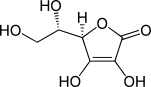
\includegraphics[width=\linewidth]{h2asc.png}
		\end{center}
	\end{minipage}
	\bigbreak
	Sur le plan chimique, c'est un diacide faible dans l'eau. Un comprimé de
	vitamine C est en fait un mélange d'acide ascorbique \ce{H2Asc} et d'ascorbate
	de sodium $(\ce{Na^+};\ce{HAsc^-})$, dans des quantités telles que la
	dissolution d'un comprimé donne un $\pH \approx \num{4.4}$ (pH de l'estomac en
	début de digestion). On admet que \textbf{ces propriétés acido-basiques ne
		jouent aucun rôle dans le dosage envisagé}.
	\bigbreak
	L'acide ascorbique possède également des propriétés réductrices~: il peut
	réduire le dioxygène. C'est pourquoi il est couramment utilisé comme
	antioxygène. Lorsqu'il est utilisé comme additif, sa présence dans les
	aliments est indiquée par le code E 300 et est limitée à \SI{300}{mg.kg^{-1}}.
	La teneur en vitamine C ou acide ascorbique dans une solution aqueuse peut
	être déterminée par un titrage direct ou indirect~; seulement, les réactions
	d'oxydoréduction dans lesquelles il intervient sont généralement lentes, de
	l'ordre de quelques minutes par équilibre.
	\begin{tcn}*(data)<ctc>{\icondata~Données}
		\begin{itemize}
			\item $E_1^\circ (\ce{S_4O_6^{2-}/S_2O_3^{2-}}) = \SI{0.08}{V}$,
			      d'équation notée (1)
			\item $E_2^\circ (\ce{Asc/H_2Asc}) = \SI{0.13}{V}$, d'équation notée (2)
			\item $E_3^\circ (\ce{I_2/I^{-}}) = \SI{0.54}{V}$, d'équation notée (3)
			\item $M(\ce{H_2Asc}) = \SI{176.1}{g.mol^{-1}}$
			\item En présence de diiode, l'empois d'amidon prend une teinte bleue
			      intense, permettant de le mettre en évidence même en très faibles
			      concentrations.
		\end{itemize}
	\end{tcn}

	\subsection{Dosage indirect par oxydoréduction}
	La méthode employée est un titrage indirect. L'acide ascorbique est mis en
	présence d'un excès \xul{connu} de diiode, et une réaction d'oxydoréduction
	totale a lieu entre les deux. On titre ensuite l'\textbf{excès} de diiode par
	une solution de thiosulfate de sodium. L'équivalence est atteinte quand il y a
	décoloration complète de la solution (avec l'empois d'amidon).
	\bigbreak
	Les solutions de diiode sont des solutions qui se conservent très mal~: nous
	avons vu dans le cours $E-\pH$ qu'il se dismute pour $\pH \gtrsim 8$. Ainsi,
	on réalisera un \textbf{titrage préliminaire} de la solution de diiode dont on
	connaît le volume $V_0$ et une approximation de la concentration $c_0$, grâce
	à la solution de thiosulfate de concentration $c_2$.
}%

\section{Analyser}
\subsection{Sécurité}

\setlist[blocQR,1]{leftmargin=10pt, label=\clenumi}
\QR{%
	\noindent
	\begin{minipage}[t]{.70\linewidth}
		On peut voir ces pictogrammes sur les étiquettes des flacons~: que
		signifient-ils~? Quelles sont les précautions à prendre~?
	\end{minipage}
	\hfill
	\begin{minipage}[t]{.25\linewidth}
		\vspace{-15pt}
		$\stackunder{\ghspic{exclam}\ghspic{aqpol}}{diiode}$
	\end{minipage}
}{%
	\begin{tasks}(2)
		\task[\hspace*{4cm}\ghspic{exclam}]\\
		Danger pour santé ou ozone~: gants, masque et lunettes.
		\task[\hspace*{2.5cm}\ghspic{aqpol}]\\
		Polluant~: attention au tri.
	\end{tasks}
}%

\subsection{Titrage préliminaire du diiode}

\QR{%
	Établir l'équation (4) du titrage du diiode par les ions thiosulfate
	$\ce{{S_2O_3}^{2-}_{\aqu}}$.
}{%
	\leavevmode\vspace*{-20pt}\relax
	\begin{align*}
		\ce{2 {S_2O_3}^2-_{\aqu} = {S_4O_6}^2-_{\aqu} + 2e^-}
		                                      & \Ra
		E_1 = E_1^\circ +
		\num{0.03} \log \frac{[\ce{S_4O_6^2-}]c^\circ}{[\ce{S_2O_3^2-}]^2}
		\tag{1}
		\\
		\ce{H_2Asc_{\aqu} = Asc + 2 {H}^+_{\aqu} + 2e^-}
		                                      & \Ra
		E_2 = E_2^\circ + \num{0.03} \log \frac{[\ce{Asc}][\ce{H^+}]^2}{[\ce{H_2Asc}]}
		\tag{2}
		\\
		\ce{2 {I}^-_{\aqu} = {I_2}_{\aqu} + 2e^-}
		                                      & \Ra
		E_3 = E_3^\circ + \num{0.03}\log \frac{{c^\circ}^2}{[\ce{I^-}]^2}
		\tag{3}
		\\
		\ce{
		{I_2}_{\aqu} + 2 {S_2O_3}^{2-}_{\aqu} & = 2 {I}^-_{\aqu} +
		{S_4O_6}^{2-}_{\aqu}
		}
		\tag*{$(4) = (3)-(1)$}
	\end{align*}
}%
\QR{%
	\label{q:c0}%
	En vous aidant d'un tableau d'avancement, trouver la relation entre $c_0$,
	$V_0$, $c_2$ et le volume équivalent $V_{\eqi,1}$.
}{%
	\leavevmode\vspace*{-15pt}\relax
	\begin{center}
		\def\rhgt{0.35}
		\centering
		\begin{tabularx}{\linewidth}{|l|c||YdYdYdY|}
			\hline
			\multicolumn{2}{|c||}{
				$\xmathstrut{\rhgt}$
			\textbf{Équation}}           &
			$\ce{{I_2}_{\aqu}}$          & $+$                  &
			$2\ce{{S_2O_3}^{2-}_{\aqu}}$ & $\ra$                &
			$2\ce{{I}^-_{\aqu}}$         & $+$                  &
			$\ce{{S_4O_6}^{2-}}$                                  \\
			\hline
			$\xmathstrut{\rhgt}$
			Initial                      & $\xi = 0$            &
			$c_0V_0$                     & \vline               &
			$C_2V$                       & \vline               &
			$0$                          & \vline               &
			$0$                                                   \\
			\hline
			$\xmathstrut{\rhgt}$
			Interm.                      & $\xi$                &
			$c_0V_0 - \xi$               & \vline               &
			$C_2V - 2\xi$                & \vline               &
			$2\xi$                       & \vline               &
			$\xi$                                                 \\
			\hline
			$\xmathstrut{\rhgt}$
			Final                        & $\xi_f = \xi_{\max}$ &
			$0$                          & \vline               &
			$0$                          & \vline               &
			$2c_0V_0$                    & \vline               &
			$c_0V_0$                                              \\
			\hline
		\end{tabularx}
	\end{center}
	\vspace{-15pt}
	\begin{gather*}
		\beforetext{À l'équivalence,}
		\xi_f = \xi\ind{max} = c_0V_0 = \frac{c_2V_{\eqi,1}}{2}
		\Lra
		\boxed{c_0 = \frac{c_2}{2}\frac{V_{\eqi,1}}{V_0}}
	\end{gather*}
}%

\subsection{Dosage en retour}
\QR{%
	Établir l'équation (5) de la réaction entre l'acide ascorbique et le diiode.
	\textbf{Démontrer} l'expression de sa constante d'équilibre et la calculer.
	Conclure sur la raison pour laquelle il convient de réaliser un titrage
	indirect. Quel aspect de la transformation de la matière n'est pas traité par
	la constante thermodynamique de la réaction~?
}{%
	\leavevmode\vspace*{-15pt}\relax
	\begin{gather*}
		\beforetext{$(5) = (3) - (2) \Ra$}
		\boxed{
		\ce{
		{I_2}_{\rm(s)} + H_2Asc = 2 {I}^-_{\aqu} + 2 {H}^+_{\aqu} + Asc
		}
		\tag*{$\DS\mathllap{K_2^\circ = \frac{[\ce{I^-}]\ind{eq}^2 [\ce{H^+}]\ind{eq}^2
			[\ce{Asc}]\ind{eq}}{[\ce{I_2}]\ind{eq}[\ce{H_2Asc}]\ind{eq}{c^\circ}^3}}$}
		}
	\end{gather*}
	On utilise l'unicité du potentiel en solution à l'équilibre pour trouver
	$K_2^\circ$~:
	\begin{gather*}
		\beforetext{$E_2 = E_3 \Lra$}
		E_3^\circ + \num{0.03} \log
		\frac{[\ce{Asc}]\ind{eq}[\ce{H^+}]\ind{eq}^2}{[\ce{H_2Asc}]\ind{eq}{c^\circ}^2}
		=
		E_2^\circ + \num{0.03} \log \frac{{c^\circ}^2}{[\ce{I^-}]\ind{eq}^2}
		\\\Lra
		\num{0.03}\log K_2^\circ = E_3^\circ-E_2^\circ
		\\\Lra
		\boxed{K_2^\circ = 10^{\DS \frac{1}{\num{0.03}} (E_3^\circ - E_2^\circ)}}
		\Ra
		\xul{K_2^\circ = 10^{\num{13.7}}}
		\quad \textbf{totale}
	\end{gather*}
	La réaction est donc thermodynamiquement favorisée et même supposée totale,
	donc elle est adaptée à un titrage direct pour ce point. En revanche, il est
	dit dans l'énoncé qu'elle est \textbf{lente}~: «~de l'ordre de quelques
	minutes par équilibre~». On ne pourrait pas réaliser un dosage colorimétrique
	précis en attendant $15 \times 2$ minutes (voire plus). Il est préférable
	\textbf{d'attendre une unique fois} que la réaction se fasse avec l'excès
	connu, puis de titrer l'excès rapidement et précisément ensuite.
	\smallbreak
	L'aspect des TM non abordé ici est évidemment la \textbf{cinétique}.
}%
\QR{%
	Soit $n_0(\ce{I_2}) = n\ind{réagi}(\ce{I_2}) + n\ind{excès}(\ce{I_2})$. En
	déduire d'abord la relation entre la quantité initiale d'acide ascorbique
	$n_0(\ce{H_2Asc})$ et $n\ind{réagi}(\ce{I_2})$, puis entre $n_0(\ce{H_2Asc})$,
	$n_0(\ce{I_2})$ et $n\ind{excès}(\ce{I_2})$.
}{%
	\leavevmode\vspace*{-15pt}\relax
	\begin{center}
		\def\rhgt{0.35}
		\centering
		\begin{tabularx}{\linewidth}{|l|c||YdYdYdYdY|}
			\hline
			\multicolumn{2}{|c||}{
				$\xmathstrut{\rhgt}$
			\textbf{Équation}}                       &
			$\ce{{I_2}_{\rm(s)}}$                    & $+$                  &
			$\ce{H_2Asc_{\aqu}}$                     & $\ra$                &
			$2\ce{{I}^-_{\aqu}}$                     & $+$                  &
			$2\ce{{H}^+_{\aqu}}$                     & $+$                  &
			$\ce{Asc_{\aqu}}$                                                 \\
			\hline
			$\xmathstrut{\rhgt}$
			Initial                                  & $\xi = 0$            &
			$n_0(\ce{I_2})$                          & \vline               &
			$n_0(\ce{H_2Asc})$                       & \vline               &
			$0$                                      & \vline               &
			$0$                                      & \vline               &
			$0$                                                               \\
			\hline
			$\xmathstrut{\rhgt}$
			Final                                    & $\xi_f = \xi_{\max}$ &
			$n_0(\ce{I_2}) - n\ind{réagi}(\ce{I_2})$ & \vline               &
			$0$                                      & \vline               &
			$2n_0(\ce{Asc})$                         & \vline               &
			$2n_0(\ce{Asc})$                         & \vline               &
			$n_0(\ce{Asc})$                                                   \\
			\hline
		\end{tabularx}
	\end{center}
	\begin{gather*}
		\beforetext{À l'équivalence~:}
		\xi_f = \xi\ind{max} = n_0(\ce{H_2Asc})
		\Lra
		\boxed{n\ind{réagi}(\ce{I_2}) = n_0(\ce{H_2Asc})}
		\\\beforetext{d'où}
		\boxed{n_0(\ce{H_2Asc}) = n_0(\ce{I_2}) - n\ind{excès}(\ce{I_2})}
	\end{gather*}
}%
\QR{%
	En utilisant l'équation (4), déterminer la relation entre l'excès de diiode et
	la quantité d'ions thiosulfate $n\ind{eqv}(\ce{S_2O_3^2-})$ versée à
	l'équivalence, notée $V\ind{eqv,2}$.
}{%
	\leavevmode\vspace*{-15pt}\relax
	\begin{gather*}
		\beforetext{Compte-tenu de la stœchiométrie,}
		\boxed{n\ind{excès}(\ce{I_2}) = \frac{c_2V\ind{eqv,2}}{2}}
	\end{gather*}
}%

\section{Réaliser}
\subsection{Étalonnage de la solution de diiode}
\enonce{%
	\begin{tcb}*(expe)<itc>"chem"{Premier titrage}
		\begin{enumerate}
			\item Introduire $V_0 = \SI{10.0}{mL}$ exactement de la solution de diiode à
			      environ \SI{5e-3}{mol.L^{-1}} dans un bécher.
			\item Titrer cette solution à l'aide du thiosulfate de sodium de
			      concentration molaire $c_2 = \SI{5.0e-3}{mol.L^{-1}}$.
			\item Ajouter quelques gouttes d'empois d'amidon lorsque la solution
			      commence à se décolorer afin d'indiquer plus précisément la fin de
			      réaction. On notera $V_{\eqi,1}$ le volume équivalent.
		\end{enumerate}
	\end{tcb}
}%

\resetQ
\setlist[blocQR,1]{leftmargin=10pt, label=\sqenumi}
\QR{%
	Faire un schéma du titrage. Vérifier sur vos précédents comptes-rendus comment
	faire un bon schéma.
}{%
	% TODO: pstricks again…
	\hfill
	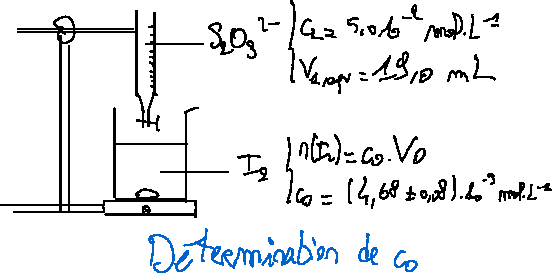
\includegraphics[width=.6\linewidth, valign=t]{det_c0}
	\hspace*{\fill}
}%
\QR{%
	Déduire de vos mesures la concentration exacte $c_0$ de la solution de diiode
	à disposition. Mettez vos valeurs en commun avec la classe, et réaliser une
	incertitude de type A pour obtenir sa valeur expérimentale (cf.\
	\url{https://capytale2.ac-paris.fr/web/c/c31b-3326128}). Comparer à la
	valeur annoncée par un écart normalisé.
}{%
	\noindent
	\begin{minipage}[t]{.27\linewidth}
		D'après~\ref{q:c0}~:
		\[
			c_0 = \frac{c_2}{2}\frac{V_{\eqi,1}}{V_0}
		\]
		On obtient les valeurs~:
	\end{minipage}
	\hfill
	\noindent
	\begin{minipage}[t]{.70\linewidth}
		\vspace{10pt}
		\begin{center}
			\begin{tabular}{ccccccccc}
				\toprule
				                             & G1         & G2         & G3         & G4        & G5 & G6 & G7 & G8
				\\
				$c_0~(\SI{e-3}{mol.L^{-1}})$ &
				\num{4.58}                   & \num{4.85} & \num{4.70} & \num{4.70} & \num{4.3} &
				\num{4.55}                   & \num{4.8}  & \num{5.0}
				\\
				\bottomrule
			\end{tabular}
		\end{center}
	\end{minipage}
	\smallbreak
	Ainsi,
	\[
		c_0 = \SI{4.68\pm 0.08e-3}{mol.L^{-1}}
		\Ra
		\xul{E_N = \num{3.16}}
	\]
	On a ainsi bien fait de la doser, puisqu'elle semble avoir bien perdu en
	concentration~!
}%

\subsection{Dosage en retour}
\enonce{%
	Vous disposez sur votre paillasse d'une solution $S_0$, obtenue en ayant
	dissout \textbf{un} comprimé de \SI{500}{mg} vitamine C dans \SI{500}{mL}
	d'eau distillée.
}%
\enonce{%
	\begin{tcb}*(expe)<itc>"chem"{Second titrage}
		\begin{enumerate}
			\item Dans un bécher, introduire \SI{5.0}{mL} de cette solution et y ajouter
			      exactement $V_1 = \SI{10.0}{mL}$ de la solution de diiode du laboratoire.
			\item Placer sous agitation magnétique pendant au moins 10 minutes.
			\item Titrer alors l'excès de diiode à l'aide de la solution de thiosulfate
			      de sodium utilisée précédemment.
			\item Ajouter quelques gouttes d'empois d'amidon lorsque la solution
			      commence à se décolorer afin d'indiquer plus précisément la fin de
			      réaction. On notera $V_{\eqi,2}$ le volume équivalent.
		\end{enumerate}
	\end{tcb}
}%
\QR{%
	Faire nouveau un schéma de cette succession de deux situations.
}{%
	% TODO: pstricks too…
	\hfill
	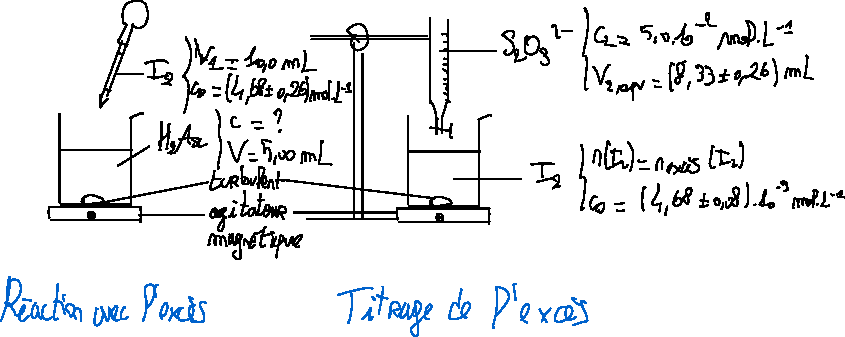
\includegraphics[width=.8\linewidth, valign=t]{tit_exces}
	\hspace*{\fill}
}%
\QR{%
	Noter l'incertitude sur le volume $V_1$ prélevé, comme indiqué sur la verrerie
	utilisée, et estimer l'incertitude sur le volume équivalent $V_{\eqi,2}$ avec
	les valeurs de la classe.
}{%
	\noindent
	\begin{minipage}[t]{.27\linewidth}
		On lit $u(V_1) = \SI[parse-numbers=false]{\frac{0.02}{\sqrt{3}}}{mL} =
			\SI{0.012}{mL}$, et on trouve les valeurs~:
	\end{minipage}
	\begin{minipage}[t]{.70\linewidth}
		\vspace{0pt}
		\begin{center}
			\begin{tabular}{ccccccccc}
				\toprule
				                         & G1        & G2        & G3        & G4        & G5 & G6 & G7 & G8
				\\
				$V\ind{2,eqv}~(\si{mL})$ &
				\num{8.5}                & \num{8.3} & \num{8.8} & \num{8.2} & \num{8.7} &
				\num{8.5}                & \num{9.0} & \num{6.6}
				\\
				\bottomrule
			\end{tabular}
		\end{center}
	\end{minipage}
	\begin{gather*}
		\beforetext{Ainsi,}
		V\ind{2,eqv} = \SI{8.33\pm 0.26e-3}{mL}
	\end{gather*}
}%

\section{Valider}
\subsection{Masse d'acide ascorbique dans un comprimé}
\QR{%
	À l'aide des relations trouvées dans la partie Analyser, donner la relation
	entre $n_0(\ce{H_2Asc})$ et les paramètres de l'étude, puis la calculer.
}{%
	\leavevmode\vspace*{-15pt}\relax
	\begin{gather*}
		\beforetext{On trouve}
		\boxed{n_0(\ce{H_2Asc}) = n\ind{réagi}(\ce{I_2}) = c_0V_1 -
			\frac{c_2V\ind{eqv,2}}{2}}
		\Ra
		\xul{n_0(\ce{H_2Asc}) = \SI{2.61e-5}{mol}}
	\end{gather*}
}%
\QR{%
	À l'aide d'une propagation des incertitudes par méthode \textsc{Monte-Carlo},
	estimer l'incertitude sur cette valeur.
}{%
	\leavevmode\vspace*{-15pt}\relax
	\[
		\xul{n_0(\ce{H_2Asc}) = \SI{2.61\pm0.10e-5}{mol}}
	\]
}%

\QR{%
	Calculer alors la quantité de matière (avec incertitude) puis la masse d'acide
	ascorbique (avec incertitude) contenue dans un comprimé. Comparer à la valeur
	annoncée \textit{via} un écart normalisé et \textbf{commenter}.
}{%
	Il y en a 100 fois plus dans le comprimé, soit
	\begin{gather*}
		\xul{n\ind{comp}(\ce{H_2Asc}) = \SI{2.61e-3}{mol}}
		\qet
		\boxed{m\ind{comp}(\ce{H_2Asc}) = n\ind{comp}(\ce{H_2Asc})M(\ce{H_2Asc})}
		\\\beforetext{d'où}
		\xul{m\ind{comp, expe}(\ce{H_2Asc}) = \SI{459\pm18}{mg}}
		\\\beforetext{or}
		\boxed{
			E_n =
			\frac{\abs{m\ind{comp, expe} - m\ind{comp, theo}}}
			{u(m\ind{compo,expe})}
		}
		\Ra
		\xul{E_n = \num{2.35}}
	\end{gather*}
	C'est limite comme correspondance, malgré un bon effort de détermination. Le
	diiode s'est peut-être encore plus dégradé entre sa mesure et son utilisation
	mais c'est peu probable. Il se peut que les excipients du comprimé
	interagissent avec la réaction, on que trop d'empois d'amidon ait été inséré.
}%

\subsection{Méthode alternative}
\QR{%
	Proposer, en le justifiant, un autre protocole indépendant permettant de doser
	l'acide ascorbique dans le comprimé. Vous pourrez chercher des valeurs de
	constantes en ligne ou les demander. Le réaliser en autonomie, et en déduire
	une seconde estimation de la masse $m$ de vitamine C dans un comprimé.
}{%
	On réalise un titrage acido-basique avec suivi pH-métrique de l'acide
	ascorbique avec de la soude, sachant que $\pk[A,1] = \num{4.1}$ et $\pk[A,2] =
		\num{11.8}$~: pour la première acidité, on trouvera
	\begin{gather*}
		\ce{H_2Asc_{\aqu} + {HO}^-_{\aqu} -> {HAsc}^-_{\aqu} + H_2O_{\rm(l)}}
		\tag*{$K^\circ = 10^{\num{9.9}}$}
	\end{gather*}
	donc bien une réaction totale. À l'équivalence, $n_0(\ce{H_2Asc}) =
		c_bV\ind{eqv,3}$, et on trouve $V\ind{eqv,3} = \SI{3.8}{mL}$.
}%

\end{document}
